\chapter{基于语料情感词典扩展}
\label{ch3}

\section{引言}
上一章内容主要介绍了进行观点分析的所需的一项基础工作,也就是通用情感词典的构建方法的研究,提出了根据语义知识库HowNet词语语义描述将英文情感词典跨语言转化为中文情感词典的自动构建方法,并构建了带有情感极性值标注的中文情感词典SentiHowNet\upcite{谢松县2014}。本章将对通用情感词典SentiHowNet在领域内进行基于语料的扩展,以增加该词典的领域覆盖度和适应性。

%自然语言中,一个词语的语义极性(semantic polarity)表示它对于其语义组(semantic group)或词汇场(lexical field)范式的偏离方向\upcite{Hatzivassiloglou1997}。在自然语言处理领域,情感分析(Sentiment Analysis)能够使用计算手段自动从自然语言中发现观点和情感等主观信息\upcite{Liu2012,Pang2008OMS},通常会使用一些标注了极性(积极或消极)的词汇构成的情感词典资源。研究如何能够通过计算方式获得词语的语义极性,自动构建情感词典一直得到计算语言学和自然语言处理研究人员关注。在英文情感词典构建中,Wilson等\upcite{Wilson2005,Wilson2009}对一些单词进行了人工极性类别的标注形成了OpinionFinder词典;Bradley等\upcite{Bradley1999}标注了并发布了情感范式的英文词典ANEW,后来Nielsen等\upcite{Nielsen2011}在Twitter语言上应用并自动扩展了ANEW,形成AFINN词典。Esuli和Sebastiani\upcite{Esuli2006}以及后来Baccianella等\upcite{Baccianella2010}在著名的语义词典Wordnet基础上采用自动计算的方式开发出了情感词典SentiWordnet。Thelwall等\upcite{Thelwall2012}设计实现了能对词语的情感强度进行估计的方法。情感也可以通过创建情绪词典来进行计算,Plutchik情绪轮提出了四对对立的情绪状态:joy-trust,sadness-anger,surprise-fear和anticipation-disgust\upcite{Plutchik2001}。Mohammad和Turney\upcite{Mohammad2013b}根据Plutchik情绪轮分类方法使用情绪分值标注了一些词语形成NRC情绪词典。在2013和2014年举办的SemEval(Semantic Evaluation)评测中,NRC-Canada队利用NRC词典并扩展出两种新的词典,取得了最好成绩\upcite{Mohammad2013,Kiritchenko2014}。为了克服以上语法层面建立的词典的上下文语境以及领域适应性问题,一些学者提出了基于概念(concept-based)构建情感词典\upcite{Tsai2013},其中SenticNet是使用常识知识库建立的公开可用的基于概念的情感词典\upcite{Cambria2014}。

基于词典的情感词典构建方法是一种常用的情感词典构建方法,采用这种方法的优势在于直接从词典中抽取情感词语,词典中词语间的显式的语义关系也有助于进行情感极性值计算。但是基于词典方法构建情感词典覆盖度受限于词典资源规模,并且只能表示词语通用的情感知识,因而在实际应用中受到多方面的挑战:一方面词典中的词语往往具有多个义项,义项之间的情感极性不尽相同,在实际应用中会存在歧义问题;另一方面,语言的词汇本身是开放的集合,会随着人类社会的发展而不断变化,尤其是对于专业领域中不断涌现的新词语,对情感词典在领域内的覆盖度提出了严峻的挑战;还有众所周知的领域适应性问题,也就是相同词语在不同的领域表达出的情感极性也会不一样。这些问题与挑战已经受到越来越多的研究者的注意\upcite{Andreevskaia2008,Choi2009,Du2010,Angel,jijkoun2010generating,Klenner2009,Qiu2009},并且提出了很多基于语料的情感词典构建方法,这些方法已在上一章的相关工作部分进行了详细介绍,在此不再赘述。随着互联网发展,尤其是社交媒体的不断涌现,越来越多的用户在各种网络平台上发布信息,网络上的各种类型用户产生内容(User Generated Content,UGC),主要包括评论(review)、博客(blogging)、微博(Twitter)以及社交网络的状态(status)等,不断涌现并以指数级速度增长。这些类型的UGC中的语言具有不同于传统媒体和知识资源的一些新特点,表达情感的词语数量上达到了新的规模,形式上发生了巨大变化,所表达的情感极性更加依赖于具体领域和语境,因此研究社交媒体中观点信息需要对在传统知识资源上构建的情感词典进行扩展,提高在UGC数据上的覆盖度以及适应性。
基于这种需求,本章提出并验证基于产品评论语料资源对SentiHowNet情感词典进行领域内的无监督扩展方法。

基于语料资源的情感词典构建方法需要解决两个问题,一是情感词语的选择,就是从语料中确定除了现有情感词典或种子词集以外的带有情感极性的词语,二是对这些词语在语料中表达的情感极性(值)进行计算。在英文中通常将这两个问题合并进行考虑,相关研究主要有两种思路:一是基于语料中文本的语言学线索,代表性研究是Hatzivassiloglou等\upcite{Hatzivassiloglou1997}基于并列或转折连词所连接词语的情感极性限制规律确定新的情感词并判断极性;二是基于语料中词语出现的上下文语境中的统计信息,代表性的研究是Turney等\upcite{Turney2002}采用点互信息(PMI)统计语料中与种子词集的词语共现度高的情感词,使用共现统计值计算其极性值。借鉴英文的情感词语选择与极性计算研究方法,本章提出基于中文语料资源对SentiHowNet情感词典扩展的三种方法,并进行实验的验证。
\begin{enumerate}
\item 基于中文语言中的并列、递进以及转折关系的连词进行情感词的发现以及极性值计算方法;
\item 统计词语在语料中上下文信息进行情感词语选择和极性值计算方法;
\item 将基于连词语言线索方法和上下文信息统计方法相结合的方式进行情感词语选择和极性计算。
\end{enumerate}

本章主要内容介绍采取与上一章不同的结构,首先介绍研究使用的词典和语料资源以及预处理,然后按照方法和实验想结合的方式分别介绍三种情感词典的扩展方法以及实验效果,最后作小节。
\section{数据集及预处理}

\subsection{词典和语料}
本章使用的词典和语料资源如表~\ref{tab3-1}所示,选取的语料资源是谭松波博士提供的酒店、书籍和电子商品三个领域评论语料\upcite{Lin2012},每个领域各有文本4000篇,其中积极极性评价和消极极性评价各2000篇。
\begin{table}[htp]
\centering
\caption{词典及语料资源}
\label{tab3-1}
\begin{tabular}{|c|l|l|}
\hline
资源 & \multicolumn{1}{c|}{名称} & \multicolumn{1}{c|}{说明} \\ \hline
词典 & SentiHowNet情感词典 & 基于上一章工作 \\ \hline
\multirow{3}{*}{语料} & 酒店(Hotel)评论 & 4000篇,积极评价和消极评价各2000篇 \\ \cline{2-3} 
 & 书籍(Book)评论 & 4000篇,积极评价和消极评价各2000篇 \\ \cline{2-3} 
 & 电脑(NoteBook)评论 & 4000篇,积极评价和消极评价各2000篇 \\ \hline
\end{tabular}
\end{table}

\subsection{数据预处理}
对数据的预处理主要包括分词与词性标注以及词语抽取形成结构化记录。
对中文文本进行深入分析前需要进行分词和词性标注,本章直接使用现有的分词工具,也就是广泛使用的中科院ICTCLAS\footnote{目前名字为NLPIR/ICTCLAS,具体见\url{http://ictclas.nlpir.org/}}分词软件\upcite{张华平2014},该工具可以对文本同时进行分词和词性标注。分词和词性标注后,过滤掉一些停用词\footnote{使用哈工大1208词的停用词表进行过滤},语料中所有的词语都有可能成为被扩展对象,因此从语料中抽取出所有词语形成结构化的记录,记录格式如图~\ref{fig3-1}所示,主要内容主要有词语编号(ID)、词性(Category)、中文词语(W\_C)、词语在句子中的编号(Word\_Tag)、词语所在语料文件编号(File\_Tag)、词语所在句子编号(Sentence\_Tag)、极性标注(Senti\_Tag)、积极极性值(PosScore)和消极极性值(NegScore)。值得说明的是,有些词在SentiHowNet中出现过,直接可以通过查询进行极性和极性值标注;极性标注的取值为Yes和No,分别表示已标注和未标注,可以用于在具体的计算过程中直接进行情感词语的选择。

\begin{figure}[htp]
\centering
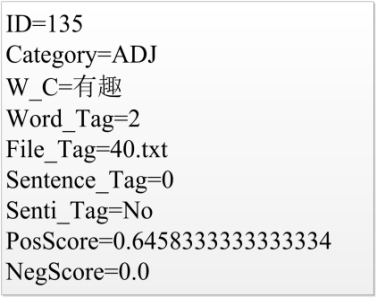
\includegraphics[height=130pt]{3-1.png}
\caption{语料预处理记录格式}
\label{fig3-1}
\end{figure}

\section{基于连词情感词典扩展}
\label{linkage}
Hatzivassiloglou等\upcite{Hatzivassiloglou1997}通过对英文语言的连词在句子中的语法和语义作用研究发现,一个句子中由连词(如and或but)连接的两个形容词或副词的情感极性存在一定的关联性,如并列连词“and”连接的两个形容词(如“nice and good”)情感极性相同,而转折连词“but”连接的两个形容词(如“nice but unnatural”)情感极性相反,否则就会引起语义上的错误(如“nice and unnatural”语法上没有问题,但是语义上不正确。)。有研究\upcite{2010}也发现中文语言也会有相同的规律,中文连词类型更丰富(有并列、转折、递进、总结、让步等类型的连词),而且数量更多,因此可以选择更多的连词进行情感词的抽取和情感极性计算。基于连词的情感词词典构建方法一般只能判断情感词的情感极性,如何能够计算得到情感词的极性强度值需要不同的方法设计。本节首先确定连词的选择,然后设计情感词语的情感极性值计算方法。

\subsection{连词选择}
连词是用来连接词与词、词组与词组或句子与句子、表示某种逻辑关系的虚词。连词可以表示并列、承接、转折、因果等关系,对连词上下文的语义倾向性有限制作用的连词一般为并列连词、转折连次以及递进连词。在此主要研究基于表达并列、转折和递进三种关系的连词如何影响情感词选择与极性值计算,通过筛选选择的连词集合为:
\begin{itemize}
\item \textbf{并列关系连词:}和、跟、与、既、同、及、况、况且、乃至、并、也、又;
\item \textbf{转折关系连词:}却、虽然、但是、然而、偏偏、只是、不过、至于、致、不料、岂知;
\item \textbf{递进关系连词:}不但、不仅、何况、并、且、而且。
\end{itemize}

\subsection{极性值计算}
SentiHowNet情感词典中的每个词都标注了情感极性值,因此语料中未标注的情感词的情感极性值可以根据所有与其在同一句子的SentiHowNet词语情感极性值计算获得。基于连词的情感词语极性计算基本思路是,对抽取到的待标注情感词语(目前仅考虑形容词和副词)所在句子进行分析,确定句子中连词及其类型,找到句子中极性值已知的情感词,并分析在句子中与连词和待标注词语的相对位置,然后依据以下原则进行计算:
\begin{enumerate}
\item 位于连词同一侧的形容词或副词具有相同极性;
\item 位于并列连词和递进连词两侧的形容词或副词具有相同极性;
\item 位于转折连词两侧的形容词或副词具有相反极性。
\end{enumerate}
对未标注词的情感值计算,对极性相同的词语情感值累加,极性相反的词语极性值相减,然后取均值。具体情感极性值计算为:
\begin{equation}
\begin{cases}
& PosScore(w_t)=\dfrac{|\sum_{w \in W_1}PosScore(w)+\sum_{w \in W_2}PosScore(w)+\sum_{w \in W_3}PosScore(w)|}{N} \\
& NegScore(w_t)=\dfrac{|\sum_{w \in W_1}NegScore(w)+\sum_{w \in W_2}NegScore(w)+\sum_{w \in W_3}NegScore(w)|}{N}
\end{cases}
\end{equation}
其中,$W_1+W_2+W_3=N$,$N$表示SentiHowNet与待标注词在同一个句子中情感词语,$W_1$,$W_2$和$W_3$分别表示与待标注词$w_t$在连接词同侧词语,在并列或递进连接词两侧词语以及在转折连接词两侧的词语。词语$w_t$极性根据积极与消极极性值大小判定为:
\begin{equation}
\label{eq3-2}
Senti\_tag(w_t)=
\begin{cases}
 positive \quad & \text{ if } PosScore(w_t)> NegScore(w_t); \\ 
 negative \quad &\text{ if } PosScore(w_t)< NegScore(w_t);  \\ 
 neutral  \quad & others
\end{cases}
\end{equation}

词语的情感极性值计算和极性判断具体过程如算法~\ref{alg3-1}所示。
\begin{algorithm}[htp]
\caption{基于连词的极性值计算}
\label{alg3-1}
\begin{algorithmic}[1]
\REQUIRE ~~\\
待标注词语集$\{w_1\}$;\\
连词集合$\{c\}$;\\
极性值已知词语集合$\{w_2\}$;
\FOR{每一待标注词语 $w_1 \in \{w_1\}$}
\FOR{每一与$\{w_1\}$在同句子中已标注词 $w_2 \in \{w_2\}$}
\IF{$\{w_1\}$和$\{w_2\}$在$c$同侧}
\STATE $
\begin{cases}
PosScore(w_1)+=PosScore(w_2)\\
NegScore(w_1)+=NegScore(w_2)
\end{cases};$
\ELSE
\IF{$c$为并列或递进连词}
\STATE $
\begin{cases}
PosScore(w_1)+=PosScore(w_2)\\
NegScore(w_1)+=NegScore(w_2)
\end{cases};$
\ENDIF
\IF{$c$为转折连词}
\STATE $
\begin{cases}
PosScore(w_1)-=PosScore(w_2)\\
NegScore(w_1)-=NegScore(w_2)
\end{cases};$
\ENDIF
\ENDIF
\ENDFOR
\STATE 计算极性均值$
\begin{cases}
PosScore(w_1)=\dfrac{|PosScore(w_1)|}{N}\\
NegScore(w_1)=\dfrac{|NegScore(w_1)|}{N}
\end{cases};$
\STATE 根据情感值 $PosScore(w_1)$ 与$ NegScore(w_1) $判断极性;
\STATE 将$ w_1 $加入到集合$ \{w_2\} $;
\ENDFOR
\end{algorithmic}
\end{algorithm}

\subsection{实验}
为了定量评价本节所提出的基于连词的情感词典扩展方法的性能,从酒店、书籍和电子商品三个领域评论语料中个随机选取了200篇评论(积极和消极极性各100篇)进行了人工标注。标注过程为:首先从评论中抽取其中的形容词和副词,过滤掉SentiHowNet中已有的词语,然后对剩余未标注词语根据在语料中的上下文标注积极和消极情感极性,标注好的词语作为评测基准。
评价指标采用精确率(P)、召回率(R)以及F值(F)作为评测指标。使用基于连词的算法抽取计算并判断极性后,在三个领域扩展得到的情感词数目统计如表~\ref{tab3-2}所示。
\begin{table}[htp]
\centering
\caption{情感词典扩展统计}
\label{tab3-2}
\begin{tabular}{|l|l|l|l|l|l|l|l|l|l|}
\hline
\multicolumn{1}{|c|}{\multirow{2}{*}{领域}} & \multicolumn{3}{c|}{积极极性} & \multicolumn{3}{c|}{消极极性} & \multicolumn{3}{c|}{总体统计} \\ \cline{2-10} 
\multicolumn{1}{|c|}{} & \multicolumn{1}{c|}{基准} & \multicolumn{1}{c|}{扩展} & \multicolumn{1}{c|}{正确} & \multicolumn{1}{c|}{基准} & \multicolumn{1}{c|}{扩展} & \multicolumn{1}{c|}{正确} & \multicolumn{1}{c|}{基准} & \multicolumn{1}{c|}{扩展} & \multicolumn{1}{c|}{正确} \\ \hline
Hotel & 103 & 88 & 75 & 98 & 124 & 98 & 201 & 212 & 173 \\ \hline
Book & 166 & 166 & 112 & 245 & 196 & 196 & 411 & 362 & 308 \\ \hline
NoteBook & 61 & 61 & 41 & 66 & 58 & 50 & 127 & 119 & 91 \\ \hline
\end{tabular}
\end{table}

从表中可以看出,在书籍领域扩展得到的情感词语较多,主要是因为书籍的评论篇幅较长,而且有更丰富的词汇来表达对书籍内容的评论,基于连词的扩展方法在消极极性词语的判断准确性较高;电子产品领域扩展的情感词较少,主要是因为对电子产品评论一般较短,表示评价观点的词汇相对比较少,专业化程度更高些,基于连词的极性计算和判断方法在该领域的准确性都比较低;而对于酒店领域基于连词的极性计算和判断方法在该领域的准确性最好。

针对三个领域的情感词典扩展实验性能评测结果如表~\ref{tab3-2-1}所示,三个语料中与上面统计相对应,基于连词的极性计算方法在酒店领域的性能最好,无论是微平均还是宏平均,精确性都高于72.82\%,在消极极性的词语精确率甚至达到100\%,召回率都高于79.03\%,F值都高于78.53\%;电子产品领域的性能指标相对较低,宏平均和微平均三个性能指标较低;在书籍领域,对消极极性情感词的判断召回率达到100\%,精确率以及F值在三个领域中都是较高,总体性能居中。从以上分析结果可以看出,基于连词的方法能够对情感词典进行有效扩展,性能较好。
\begin{table}[htp]
\centering
\caption{性能评测结果}
\label{tab3-2-1}
\begin{tabular}{|l|l|l|l|l|l|l|l|l|l|}
\hline
\multicolumn{1}{|c|}{\multirow{2}{*}{领域}} & \multicolumn{3}{c|}{积极极性} & \multicolumn{3}{c|}{消极极性} & \multicolumn{3}{c|}{宏平均} \\ \cline{2-10} 
\multicolumn{1}{|c|}{} & \multicolumn{1}{c|}{P} & \multicolumn{1}{c|}{R} & \multicolumn{1}{c|}{F} & \multicolumn{1}{c|}{P} & \multicolumn{1}{c|}{R} & \multicolumn{1}{c|}{F} & \multicolumn{1}{c|}{P} & \multicolumn{1}{c|}{R} & \multicolumn{1}{c|}{F} \\ \hline
Hotel & 0.7282 & 0.8523 & 0.7853 & 1.0000 & 0.7903 & 0.8829 & 0.8607 & 0.8160 & 0.8378 \\ \hline
Book & 0.6747 & 0.6747 & 0.6747 & 0.8000 & 1.0000 & 0.8889 & 0.7494 & 0.8508 & 0.7969 \\ \hline
NoteBook & 0.6721 & 0.6721 & 0.6721 & 0.7576 & 0.8621 & 0.8065 & 0.7165 & 0.7647 & 0.7398 \\ \hline
\end{tabular}
\end{table}

\section{基于上下文情感词典扩展}
词语的上下文是词语在实际应用中的语言环境,对于词语的语义理解有着重要作用,是自然语言处理经常使用的信息,它在自然语言处理中的价值体现在两个方面:一方面,在自然语言知识获取的过程中,上下文是知识获取的重要来源;另一方面,在自然语言处理的具体应用问题解决过程中,上下文扮演着问题所需信息和资源提供者的重要角色。特别是在语料库语言学中,各种机器学习方法的引入使词语的上下文成为计算语言学知识获取和问题求解过程中最为重要的资源,在无监督学习方法中更是如此\upcite{鲁松2001}。对于本章要解决的情感词语抽取和极性值计算任务来说,统计情感词语出现的上下文特征可以为情感极性值的计算提供有用信息,因为出现在相同上下文环境中的词语具有相似的情感极性。

上下文的选取是基于核心词左右一定范围进行的,这个固定的范围被称为“窗口”。选择合适的窗口,可以为基于上下文信息的计算方法提供的信息量足够大,产生的噪声足够小。在英文中,核心词左右5个词的范围可以为词语搭配提供95\%的信息,上下文±2是最好的选择,范围进一步扩大后提供的信息量不会有明显的增加且会带来不必要的计算开销\upcite{Yarowsky1993,Martin1983}。

词语的上下文可以利用的信息有很多,一般是直接将上下文中出现的词作为有效特征使用\upcite{Sinclair1991,张猛2008},但是这种方法需要面临的一个问题是上下文特征的稀疏性,尤其是对社交媒体文本来说,篇幅一般较短,而且词语的不规范使用现象普遍,稀疏问题会更严重。因此本节采用了上下文词语的词性信息进行统计和计算。具体来讲,首先是对待标注情感词语,分析上下文中词语的词性,获取一个词性特征向量,然后根据其上下文特征向量进行词语情感极性值计算。

\subsection{上下文特征向量}
对于词语$w$,通过分析在一定窗口范围内上下文中词语的词性形成词语的特征向量,下面给出形式化定义。
\begin{definition}[词语$w$的特征向量$V(w)$和窗口$W$]
词语$w$的特征向量$V(w)$是指由词语$w$与其相邻上下文词语的词性组成的向量,具体形式为:
$$V(w)=<C_{-W},C_{-W+1},\cdots C_{-1},C_0,C_{W-1},C_W>$$
其中,$C_0$表示词语$w$的词性,$C_i(i\neq 0)$表示与$w$相邻的词语的词性,$i$表示与词语$w$的相对距离,$W$表示窗口,即特征向量中与词语$w$相对距离的最大值。
\end{definition}

\subsection{基于词性特征向量的极性值计算}
基于上下文的情感词极性值计算的基本假设就是具有相同的上下文特征向量的词语具有相同的极性,根据这一假设,统计出SentiHowNet中与待标注词$ w_t$词性特征向量相同的情感词,然后计算$ w_t $的情感极性值。如果待标注词$ w_t$出现的上下文中有$ N $中词性特征向量,则$ w_t$的情感极性值计算公式为:
\begin{equation}
\label{eq3-2-1}
\begin{cases}
PosScore(w_t)=\dfrac{\sum_{V(w)=V(w_t)}\dfrac{|\sum_{w \in W_{positive}}PosScore(w)-\sum_{w \in W_{negative}}PosScore(w)|}{|M|}}{|N|} \\
NegScore(w_t)=\dfrac{\sum_{V(w)=V(w_t)}\dfrac{|\sum_{w \in W_{positive}}NegScore(w)-\sum_{w \in W_{negative}}NegScore(w)|}{|M|}}{|N|} \\
\end{cases}
\end{equation}
其中$W_{positive}+W_{negative}=M$,表示与待标注词$w_t$具有同一特征向量$ V(w_t) $的SentiHowNet中的情感词集,$W_{positive}$和$W_{negative}$分别为极性为积极和消极的词语。$w_t$极性判断依据其积极与消极极性值的大小判断,同公式~\ref{eq3-2}。

以书籍语料中形容词“亮丽”为例,设定$ W=2 $,在语料中抽取“亮丽”所有的$ N $种词性特征向量,其中的一个的特征向量为$ <daaun> $,从SentiHowNet中获取与“亮丽”的这一词性特征向量相同的所有情感词如表~\ref{tab3-3-1}所示,共有16个情感词与“亮丽”有相同的词性特征向量$ <daaun> $,其中积极极性词语10个,消极极性词语5个,于是可以使用公式~\ref{eq3-2-1}计算其情感极性值为积极极性值为0.4297,消极极性值0.0421。当然这是词性特征向量$ <daaun> $计算出的极性值,将所有$ N $种词性特征向量计算的极性值取平均就可以得到“亮丽”在书籍领域最终情感极性值。
\begin{table}[htp]
\centering
\caption{计算示例}
\label{tab3-3-1}
\begin{tabular}{|l|l|l|l|}
\hline
\multicolumn{1}{|c|}{情感词} & \multicolumn{1}{c|}{情感词上下文} & \multicolumn{1}{c|}{情感词} & \multicolumn{1}{c|}{情感词上下文} \\ \hline
大 & 没有多大的可读性 & 弱小 & 再贫困弱小的人 \\ \hline
简单 & 太浅显简单的东西 & 有趣 & 又生动有趣的绘画 \\ \hline
真实 & 比较客观真实的角度 & 直观 & 没有明显直观的效益 \\ \hline
新鲜 & 更多新鲜的元素 & 奇妙 & 更多奇妙的东西 \\ \hline
严格 & 太多严格的界限 & 好 & 更多好的作品 \\ \hline
石破天惊 & 颇多石破天惊之语 & 肮脏 & 太多肮脏的东西 \\ \hline
柔软 & 最脆弱柔软的心脏 & 多 & 反正好多的故事 \\ \hline
粗俗 & 原本低级粗俗的俚语 & 曲折 & 明明惊险曲折的战争 \\ \hline
\end{tabular}
\end{table}

更一般的,基于词性特征向量的情感极性值具体计算过程如算法~\ref{alg3-2}所示。

\begin{algorithm}[htp]
\caption{基于统计特征的极性计算}
\label{alg3-2}
\begin{algorithmic}[1]
\REQUIRE ~~\\
待标注词语集$\{w_1\}$;\\
极性已知词语集合$\{w_2\}$;\\
每个词特征向量集合$\{V(w)|w \in \{w_1\}\cup \{w_2\} \}$;
\FOR{每一待标注词语 $w_1 \in \{w_1\}$}
\FOR{$w_1$每一特征向量$V(w_1)$}
\FOR{每一与$V(w_1)  $相同的特征向量$ \{V(w_1)=V(w_2)|w_2 \in \{w_2\} \}$}
\IF{$Senti_Tag(w_2)=positive$}
\STATE $
\begin{cases}
PosScore(w_1)+=PosScore(w_2)\\
NegScore(w_1)+=NegScore(w_2)
\end{cases};$
\ELSE
\STATE $
\begin{cases}
PosScore(w_1)-=PosScore(w_2)\\
NegScore(w_1)-=NegScore(w_2)
\end{cases};$
\ENDIF
\ENDFOR
\STATE 对各个特征向量下的情感值累加
\STATE $
\begin{cases}
PosScore(w_1)+=PosScore(w_1)\\
NegScore(w_1)+=NegScore(w_1)
\end{cases};$
\ENDFOR
\STATE 计算极性均值$
\begin{cases}
PosScore(w_1)=\dfrac{PosScore(w_1)}{i}\\
NegScore(w_1)=\dfrac{NegScore(w_2)}{i}
\end{cases};$
\STATE 根据情感值 $PosScore(w_1)$ 与$ NegScore(w_1) $判断极性;
\STATE 将$ w_1 $加入到集合$ \{w_2\} $;
\ENDFOR
\end{algorithmic}
\end{algorithm}

\subsection{实验}
评测实验使用的数据、基准与评测指标与基于连词的方法~\ref{linkage}节相同。
对三个领域的情感词典扩展实验结果如图~\ref{fig3-2}、图~\ref{fig3-3}和图~\ref{fig3-4}所示,三个图中分别显示了精确率、召回率以及F值的积极和消极极性的宏平均结果。图中可以看出当窗口$W=1$时,在三个领域的数据中,基于词性特征向量方法都能够准确抽取所有的情感词,因此精确率、召回率以及F值相同,分别为67.65\%、72.89\%和72.13\%;当窗口增加到$W=2$时,召回率都略有上升,精确率都有所下降,酒店领域基本不变,书籍领域下降6.62\%,电子产品领域下降最多(8.1\%),F值都变化不大;当窗口增加到$W=3$时,除酒店领域的召回率上升外,其他两个领域和其他指标都出现明显下降。因此通过分析各个领域的性能指标,采用上下文窗口$W=2$时,基于词性特征向量的情感值计算方法性能最好,这与在英文领域的研究结论\upcite{Yarowsky1993,Martin1983}是一致的。

\begin{figure}[htp]
\centering
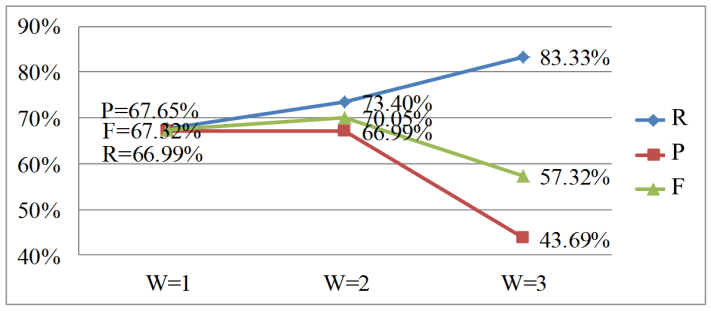
\includegraphics[height=150pt]{3-2.png}
\caption{Hotel语料评测结果}
\label{fig3-2}
\end{figure}

\begin{figure}[htp]
\centering
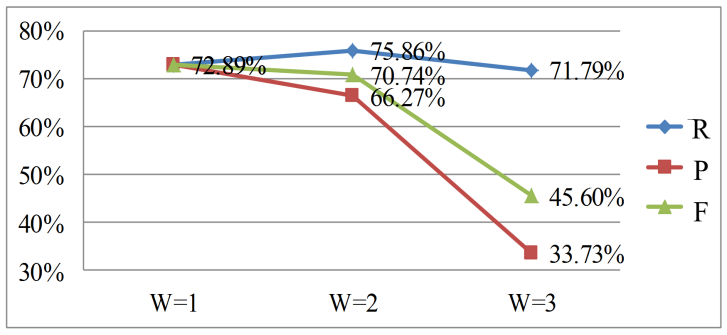
\includegraphics[height=150pt]{3-3.png}
\caption{Book语料评测结果}
\label{fig3-3}
\end{figure}

\begin{figure}[htp]
\centering
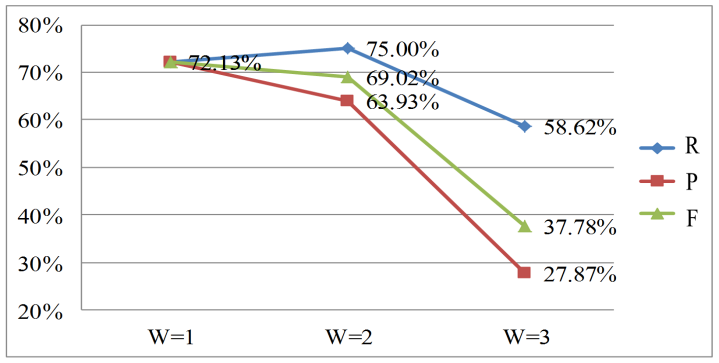
\includegraphics[height=170pt]{3-4.png}
\caption{NoteBook语料评测结果}
\label{fig3-4}
\end{figure}

当窗口$W=2$时在三个领域扩展得到的情感词数目统计如表~\ref{tab3-2-3}所示。
\begin{table}[htp]
\centering
\caption{情感词典扩展统计}
\label{tab3-2-3}
\begin{tabular}{|l|l|l|l|l|l|l|l|l|l|}
\hline
\multicolumn{1}{|c|}{\multirow{2}{*}{领域}} & \multicolumn{3}{c|}{积极极性} & \multicolumn{3}{c|}{消极极性} & \multicolumn{3}{c|}{总体统计} \\ \cline{2-10} 
\multicolumn{1}{|c|}{} & \multicolumn{1}{c|}{基准} & \multicolumn{1}{c|}{扩展} & \multicolumn{1}{c|}{正确} & \multicolumn{1}{c|}{基准} & \multicolumn{1}{c|}{扩展} & \multicolumn{1}{c|}{正确} & \multicolumn{1}{c|}{基准} & \multicolumn{1}{c|}{扩展} & \multicolumn{1}{c|}{正确} \\ \hline
Hotel & 103 & 98 & 64 & 98 & 86 & 71 & 201 & 184 & 135 \\ \hline
Book & 166 & 128 & 115 & 245 & 231 & 157 & 411 & 359 & 272 \\ \hline
NoteBook & 61 & 50 & 42 & 66 & 58 & 39 & 127 & 108 & 81 \\ \hline
\end{tabular}
\end{table}

\section{基于混合方法情感词典扩展}
对基于词性特征向量的情感词典扩展方法的实验结果分析发现,在统计词语的上下文词性特征向量时,有些词在SentiHowNet中没有发现与之词性特征向量相同的情感词,无法采用基于词性特征向量方法计算情感极性值,这种情况下可以考虑采用基于连词的方法进行计算。同样的,对基于连词的情感词典扩展方法实验结果分析发现,在语料中有些情感词出现的所有句子中没有任何并列、递进或者转折连词出现,无法采用基于连词方法计算情感极性值,这种情况下可以考虑采用基于词语上下文的词性特征向量方法进行计算。两种方法可以相互补充,因此本节提出将两中方法混合使用的方法,并实验验证混合方法的性能。

\subsection{基于混合方法的极性值计算}
对任一选取的情感词$ w $,分别采用两种方法进行极性值计算,在将两种方法计算的极性值合成时,遵循以下原则:
\begin{enumerate}
\item 优先采用基于词性特征向量的方法计算出的情感极性值作为待标注词语的情感极性值。
\item 当采用基于词性特征向量的方法进行计算时,优先设置上下文窗口大小为2,其次为1。
\item 当采用基于词性特征向量的方法无法对待标注词语进行情感值计算时,采用基于连词的方法进行计算。
\end{enumerate}

具体的混合方法计算情感词语极性值如算法~\ref{alg3-3}所示。
\begin{algorithm}[htp]
\caption{基于混合特征的极性计算}
\label{alg3-3}
\begin{algorithmic}[1]
\REQUIRE ~~\\
待标注词语集$\{w_1\}$;\\
极性已知词语集合$\{w_2\}$;\\
连词集合$\{c\}$;\\
每个词特征向量集合$\{V(w)|w \in \{w_1\}\cup \{w_2\} \}$;

\FOR{每一待标注词语 $w_1 \in \{w_1\}$}
\STATE 依据算法~\ref{alg3-2}计算情感极性值
\IF{$
\begin{cases}
PosScore(w_1)=0\\
NegScore(w_1)=0
\end{cases}$}
\STATE 依据算法~\ref{alg3-1}计算情感极性值
\ENDIF
\STATE 根据情感值 $PosScore(w_1)$ 与$ NegScore(w_1) $判断极性;
\STATE 将$ w_1 $加入到集合$ \{w_2\} $;
\ENDFOR
\end{algorithmic}
\end{algorithm}

\subsection{实验}
基于混合方法评测实验使用的数据、基准与评测指标与基于连词的方法~\ref{linkage}节相同。
在三个领域扩展得到的情感词数目统计如表~\ref{tab3-3}所示。与表~\ref{tab3-2-3}以及表~\ref{tab3-2}进行对比,可以看出基于混合方法在每个领域的正确标注词数目比基于连词和基于词性特征向量的方法都有明显增加。
\begin{table}[htp]
\centering
\caption{情感词典扩展统计}
\label{tab3-3}
\begin{tabular}{|l|l|l|l|l|l|l|l|l|l|}
\hline
\multicolumn{1}{|c|}{\multirow{2}{*}{领域}} & \multicolumn{3}{c|}{积极极性} & \multicolumn{3}{c|}{消极极性} & \multicolumn{3}{c|}{总体统计} \\ \cline{2-10} 
\multicolumn{1}{|c|}{} & \multicolumn{1}{c|}{基准} & \multicolumn{1}{c|}{扩展} & \multicolumn{1}{c|}{正确} & \multicolumn{1}{c|}{基准} & \multicolumn{1}{c|}{扩展} & \multicolumn{1}{c|}{正确} & \multicolumn{1}{c|}{基准} & \multicolumn{1}{c|}{扩展} & \multicolumn{1}{c|}{正确} \\ \hline
Hotel & 103 & 103 & 64 & 98 & 100 & 88 & 201 & 203 & 152 \\ \hline
Book & 166 & 175 & 125 & 245 & 236 & 192 & 411 & 411 & 317 \\ \hline
NoteBook & 61 & 66 & 48 & 66 & 61 & 52 & 127 & 127 & 100 \\ \hline
\end{tabular}
\end{table}

对三个领域(Hotel、Book、NoteBook)的情感词典扩展实验精确率、召回率以及F值的微平均及宏平均结果如表~\ref{tab3-4}所示。表中可以看出,基于混合方法在三个领域的性能指标都比较稳定,宏平均的精确率、召回率以及F值都在74\%以上,电子产品领域性能最好(三个指标都达到78.69\%),酒店领域稍低,数据领域居中。
\begin{table}[htp]
\centering
\caption{各个领域性能评测结果}
\label{tab3-4}
\begin{tabular}{|l|l|l|l|l|l|l|l|l|l|}
\hline
\multicolumn{1}{|c|}{\multirow{2}{*}{领域}} & \multicolumn{3}{c|}{积极极性} & \multicolumn{3}{c|}{消极极性} & \multicolumn{3}{c|}{宏平均} \\ \cline{2-10} 
\multicolumn{1}{|c|}{} & \multicolumn{1}{c|}{P} & \multicolumn{1}{c|}{R} & \multicolumn{1}{c|}{F} & \multicolumn{1}{c|}{P} & \multicolumn{1}{c|}{R} & \multicolumn{1}{c|}{F} & \multicolumn{1}{c|}{P} & \multicolumn{1}{c|}{R} & \multicolumn{1}{c|}{F} \\ \hline
Hotel & 0.6214 & 0.6214 & 0.6214 & 0.8980 & 0.8800 & 0.8889 & 0.7549 & 0.7476 & 0.7512 \\ \hline
Book & 0.7837 & 0.8136 & 0.7983 & 0.7530 & 0.7143 & 0.7331 & 0.7711 & 0.7711 & 0.7711 \\ \hline
NoteBook & 0.7869 & 0.7273 & 0.7559 & 0.7879 & 0.8525 & 0.8189 & 0.7869 & 0.7869 & 0.7869 \\ \hline
\end{tabular}
\end{table}

为了综合比较本章的三种方法,基于连词的情感词典扩展、基于词性特征向量的情感词典扩展和混合方法的情感词典扩展的实验评测宏平均结果对比情况如图~\ref{fig3-5}、图6~\ref{fig3-6}和图~\ref{fig3-7}所示,从比较结果来看,混合方法在性能是在三个领域语料中均是最优的,是比较理想的情感词典扩展方法,其次为基于词性特征向量的方法(取窗口为2时),基于连词方法性能接近于词性特征向量的方法。因此在选择对SentiHowNet情感词典扩展方法时,优先选择混合方法。

\begin{figure}[htp]
\centering
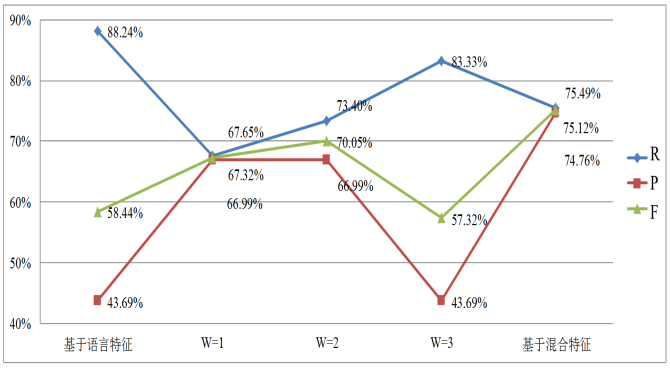
\includegraphics[height=200pt]{3-5.png}
\caption{Hotel语料评测结果综合比较}
\label{fig3-5}
\end{figure}

\begin{figure}[htp]
\centering
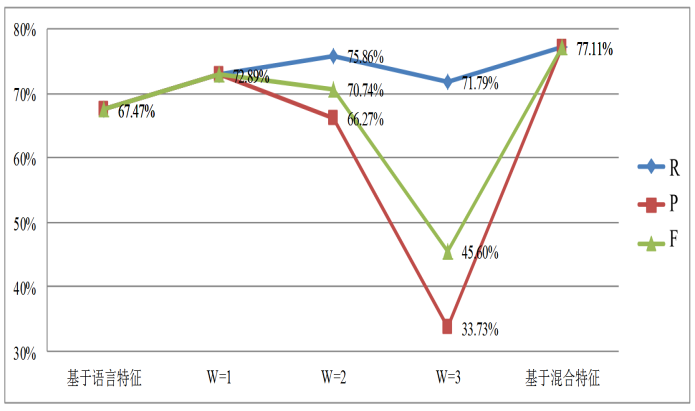
\includegraphics[height=200pt]{3-6.png}
\caption{Book语料评测结果综合比较}
\label{fig3-6}
\end{figure}

\begin{figure}[htp]
\centering
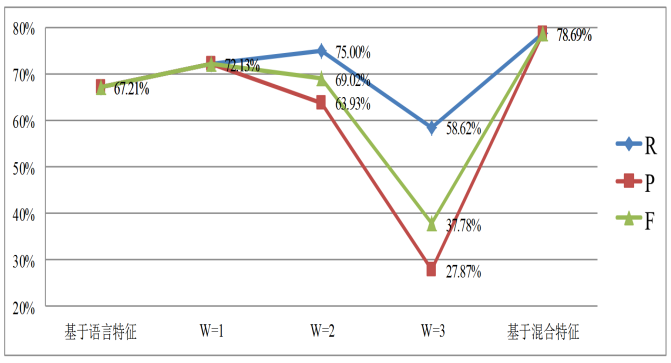
\includegraphics[height=200pt]{3-7.png}
\caption{NoteBook语料评测结果综合比较}
\label{fig3-7}
\end{figure}

\section{小结}
本章详细讨论了基于语料资源的中文情感词典的三种扩展方法,并用三个领域的评论语料进行了实验验证。第一种方法是基于连词语言线索方法,该方法根据语言中连词对词语语义倾向的限制作用,选择了并列、转折以及递进三类连词来进行词典扩展,设计了基于连词的情感词的极性值计算方法以及详细算法,实验验证了中文连词在情感词典扩展中的有效作用;第二种方法是基于词性特征向量的方法,根据出现在相同上下文的词语语义倾向性的相似性,设计词语的词性特征向量,统计具有相同词性特征向量的情感词进行情感极性值计算,并设计了详细算法,实验结果证明了词性特征向量的有效性;第三种方法为前两种方法的混合,可以利用两种方法间相互补充的作用提高情感词的识别以及极性值计算准确性,实验结果证明混合方法在三种方法中在三个领域中最为稳定,性能最好。

